\documentclass{article}
%
\usepackage[mathcal,mathbf]{euler}
\usepackage{theorem,amsmath,enumerate,fancyhdr,amssymb,amsfonts}
\usepackage[pdftex]{graphics}
\usepackage{graphicx}

\usepackage{myDefs}

\begin{document}

\pagestyle{fancy}
\lhead{{\bf Assignment 1}
\\{\bf Author: }{Yuan Qu} } 
\rhead{{\bf Date: }01/31/2017} 

\section*{Question 1}{
    \subsection*{a.}{
        This defines an independence system \((\mathit{E},\mathcal{F}), \mathcal{F} \subseteq \mathrm{2}^{\mathit{E}}\)\\

        First, prove that \(\emptyset \in \mathcal{F}\).

        Obviously, we have \(\emptyset \subseteq \mathit{E}=\{\mathrm{1,2,...,n}\}\), and \(\mathit{a}(\emptyset)=\sum_{\mathit{j} \in \emptyset}=\mathrm{0} \leqslant \mathit{b} \in \mathbb{R}_{+}\)

        So, \(\emptyset \in \mathcal{F}\).\\

        Second, prove that \(\mathit{X} \subseteq \mathit{Y} \in \mathcal{F} \Rightarrow \mathit{X} \in \mathcal{F}\)

        \[\mathit{Y} \in \mathcal{F} \Rightarrow \mathit{a}(\mathit{Y}) = \sum_{\mathit{j} \in \mathit{Y}}\mathit{a_j} \leqslant \mathit{b}\]

        \[\mathit{X} \subseteq \mathit{Y} \Rightarrow \mathit{a}(\mathit{X}) = \sum_{\mathit{j} \in \mathit{X}}\mathit{a_j} = \sum_{\mathit{i} \in \mathit{Y}}\mathit{a_i} - \sum_{\mathit{j} \in \mathit{Y} \setminus \mathit{X}}\mathit{a_j} \leqslant \sum_{\mathit{j} \in \mathit{Y}}\mathit{a_j} \leqslant \mathit{b}\]\\

        So, this difines an independence system \((\mathit{E},\mathcal{F}), \mathcal{F} \subseteq \mathrm{2}^{\mathit{E}}\)
    }
    \subsection*{b.}{
        According to the defination, we have
        \[\mathrm{n=6} \Rightarrow \mathit{S} \subseteq \mathit{E} = \{ \mathrm{1,2,3,4,5,6}\}\]
        \[\mathit{a}=\mathrm{(1,1,1,4,4,5), b=8} \Rightarrow \mathit{a}(\mathit{S}) = \sum_{\mathit{j} \in \mathit{S}}\mathit{a_j} \leqslant \mathrm{8}\]
        According to the defination of \textit{rank}, we have
        \[\mathit{r(X)}=\underset{\mathit{F} \in \mathcal{F}}{\mathit{max}} \lvert \mathit{F} \cap \mathit{X} \rvert=\underset{\mathit{B} \in \mathcal{B}_{\mathit{X}}} {\mathit{max}} \lvert \mathit{B} \rvert \text{, and } \mathit{\rho(X)} = \underset{\mathit{B} \in \mathcal{B}_{\mathit{X}}} {\mathit{min}} \lvert \mathit{B} \rvert\]
        We can find that
        \[\mathcal{B}_{\mathit{X}} = \mathrm{\big{\{} \{1,2,3,4\}, \{1,2,3,5\}, \{1,2,3,6\}, \{4,5\}\big{\}}}\]
        So that we have \(\mathit{r(X)}=\mathrm{4}, \mathit{\rho(X)}=\mathrm{2}\)
    }
    \subsection*{c.}{
        \[\mathit{O\big{(}r(X)\big{)}=O(n log n)}\]
        As the greedy algorithm, order the \(\mathit{a}\) from small to large, use the \textit{Best-in Greedy} to select numbers from the smallest. So the complexity is \(\mathit{O(n log n)}\)
    }
    \subsection*{d.}{
        \[\mathit{O\big{(}\rho(X)\big{)}=O(n^{\mathrm{2}})}\]
        Need to find all the subset of \(\mathit{S}\) So the complexity is \(\mathit{O(n^2)}\)
    }
    \subsection*{e.}{
        As \textit{b.} mentioned, \(\mathit{B}_{\mathrm{3}}=\mathrm{\{1,2,3,6\}},\mathit{B}_{\mathrm{4}}=\mathrm{\{4,5\}}\). If we use \textit{Best-in Greedy}, we may lose the \(\mathit{B}_{\mathrm{4}}\), because there is a solution when the first choice is 6. 
    }
}

\section*{Question 2}{
    \subsection*{a.}{
        We have the job set \(\mathit{E}\) like following
        \begin{center}{
            \begin{tabular}{|c|c|c|c|c|c|c|c|}
            \hline
            Job & 1 & 2 & 3 & 4 & 5 & 6 & 7 \\
            \hline
            Due & 3 & 2 & 4 & 1 & 4 & 4 & 6 \\
            \hline
            Profit & 2 & 3 & 4 & 3 & 3 & 6 & 7 \\
            \hline
            \end{tabular}
        }
        \end{center} 
        The purpose is to find a independent subset \(\mathit{S} \subseteq \mathit{E}\)\\
        The initialization of \textit{Best-in Greedy} is sorting the jobs, as following
        \begin{center}{
            \begin{tabular}{|c|c|c|c|c|c|c|c|}
            \hline
            Job & 7 & 6 & 3 & 5 & 4 & 2 & 1 \\
            \hline
            Due & 6 & 4 & 4 & 4 & 1 & 2 & 3 \\
            \hline
            Profit & 7 & 6 & 4 & 3 & 3 & 3 & 2 \\
            \hline
            \end{tabular}
        }
        \end{center} 
        Then, as \textit{Best-in Greedy}, the process would be
        \begin{center}{
            \begin{tabular}{|c|c|c|c|c|}
            \hline
            Date & 1 & 2 & 3 & 4 \\
            \hline
            Job & 7 & 6 & 3 & 5 \\
            \hline
            Due & 6 & 4 & 4 & 4 \\
            \hline
            Profit & 7 & 6 & 4 & 3 \\
            \hline
            \end{tabular}
        }
        \end{center}
        The total profit would be: \(\mathrm{7+6+4+3=20}\)
    }
    \subsection*{b.}{
        Suppose \(\mathit{A}\) and \(\mathit{B}\) are two independent subsets of \(\mathit{E}\), so we have \(\mathit{A}, \mathit{B} \subseteq \mathit{E}\), and \(\mathit{A}, \mathit{B} \in \mathcal{F}\). Construct \(\mathit{A}\) and \(\mathit{B}\) as:

        \[\mathit{A}=\{ \mathit{a}_{\mathrm{1}}, \mathit{a}_{\mathrm{2}}, ..., \mathit{a}_{\mathrm{k}}\}, \mathit{B}=\{ \mathit{b}_{\mathrm{1}}, \mathit{b}_{\mathrm{2}}, ..., \mathit{b}_{\mathrm{m}}\}, \mathit{a}_{\mathrm{i}} \text{ and } \mathit{b}_{\mathrm{j}} \text{ means the job in }\mathit{A}, \mathit{B}\]

        Suppose that \(\mathrm{k} < \mathrm{m}\), so \(\lvert \mathit{A} \rvert < \lvert \mathit{B} \rvert\).

        If all the due of \(\mathit{a}_{\mathrm{i}}\) is less or equal than \(\mathrm{k}\), it's easy to find a \(\mathit{b}_{\mathrm{j}}\) whose due is larger than \(\mathrm{k}\), because of \(\mathrm{k} < \mathrm{m}\). So, we can add \(\mathit{b}_{\mathrm{j}}\) to \(\mathit{A}\) as \(\mathit{a}_{\mathrm{k+1}}\) and all the jobs can be processed, 
        \[\mathit{b}_{\mathrm{j}} \in \mathit{B} \setminus \mathit{A}, \mathit{A} \cup \{ \mathit{b}_{\mathrm{j}} \} \in \mathcal{F}\]

        If \(\exists \mathit{a}_{\mathrm{i}}, \mathit{d}_{\mathit{a}_{\mathrm{i}}}>k\), we can find a \(\mathit{b}_{\mathrm{j}} \in \mathit{B} \setminus \mathit{A}\) whose due is larger than \(\mathrm{i}\), because of \(\mathrm{k-i} < \mathrm{m-i}\). So, we can put \(\mathit{a}_{\mathrm{i}}\) as \((\mathrm{k+1})\)th process and set \(\mathit{b}_{\mathrm{j}}\) as \(\mathrm{i}\)th process, all the jobs can be processed,
        \[\mathit{b}_{\mathrm{j}} \in \mathit{B} \setminus \mathit{A}, \mathit{A} \cup \{ \mathit{b}_{\mathrm{j}} \} \in \mathcal{F}\]

        So, \((\mathit{E},\mathcal{F})\) is a matroid.
    }
}

\section*{Question 3}{
    \subsection*{a.}{
        \(\big{(}\mathit{V(G)},\mathcal{F}\big{)}\) is a matroid.\\

        First, prove that \(\emptyset \in \mathcal{F}\).

        Obviously, we have \(\emptyset \subseteq \mathit{V(G)}\), and there is no edge because of no vertex. 

        So, \(\emptyset \in \mathcal{F}\).\\

        Second, prove that \(\mathit{X} \subseteq \mathit{Y} \in \mathcal{F} \Rightarrow \mathit{X} \in \mathcal{F}\)

        If \(\mathit{Y}\) is independent, which means no edge inside the \(\mathit{Y}\), obviously all the subsets of \(\mathit{Y}\) contain no edge inside.

        So, this difines an independence system \(\big{(}\mathit{V(G)},\mathcal{F}\big{)}, \mathcal{F} \subseteq \mathrm{2}^{\mathit{V(G)}}\)\\

        Third, to prove that the independence system \(\big{(}\mathit{V(G)},\mathcal{F}\big{)}\) is a matroid, according to the \textit{lemma 2}, only need to prove \textbf{for each \(\mathit{X} \subseteq \mathit{E}\), all bases of \(\mathit{X}\) are of the same size.}

        Supposed \(\lvert \mathit{V(G)} \rvert = \mathrm{n}\). 

        Apparently, no matter which vertices are chosen, for \(\mathrm{n}\) is \textit{odd}, the size of all the bases of \(\mathit{X}\) is equal to \(\frac{\mathit{n}-\mathrm{1}}{\mathrm{2}}\), and for \(\mathrm{n}\) is \textit{even}, the size of all the bases of \(\mathit{X}\) is equal to \(\frac{\mathit{n}}{\mathrm{2}}\).\\

        So, \(\big{(}\mathit{V(G)},\mathcal{F}\big{)}\) is a matroid.
    }
    \subsection*{b.}{
        While \(\mathit{n} = \mathrm{5}\), according to \textit{a.}, so that the size of bases \(\mathit{r(S)} = \frac{\mathit{n}-\mathrm{1}}{\mathrm{2}}=\mathrm{2}\).

        Therefore, the defining inequalities for \(\mathit{P}_{\mathit{V(G)},\mathcal{F}}\):

        \[\mathit{S}_{\mathrm{1}} = \{ \mathit{x}_{\mathrm{1}}, \mathit{x}_{\mathrm{3}}\} \quad \mathit{x}(\mathit{S}_{\mathrm{1}}) = \mathit{x}_{\mathrm{1}} + \mathit{x}_{\mathrm{3}} \leqslant \mathit{r(S)} = 2\]

        \[\mathit{S}_{\mathrm{2}} = \{ \mathit{x}_{\mathrm{2}}, \mathit{x}_{\mathrm{4}}\} \quad \mathit{x}(\mathit{S}_{\mathrm{2}}) = \mathit{x}_{\mathrm{2}} + \mathit{x}_{\mathrm{4}} \leqslant \mathit{r(S)} = 2\]

        \[\mathit{S}_{\mathrm{3}} = \{ \mathit{x}_{\mathrm{3}}, \mathit{x}_{\mathrm{5}}\} \quad \mathit{x}(\mathit{S}_{\mathrm{3}}) = \mathit{x}_{\mathrm{3}} + \mathit{x}_{\mathrm{5}} \leqslant \mathit{r(S)} = 2\]

        \[\mathit{S}_{\mathrm{4}} = \{ \mathit{x}_{\mathrm{4}}, \mathit{x}_{\mathrm{1}}\} \quad \mathit{x}(\mathit{S}_{\mathrm{4}}) = \mathit{x}_{\mathrm{4}} + \mathit{x}_{\mathrm{1}} \leqslant \mathit{r(S)} = 2\]

        \[\mathit{S}_{\mathrm{5}} = \{ \mathit{x}_{\mathrm{5}}, \mathit{x}_{\mathrm{2}}\} \quad \mathit{x}(\mathit{S}_{\mathrm{5}}) = \mathit{x}_{\mathrm{5}} + \mathit{x}_{\mathrm{2}} \leqslant \mathit{r(S)} = 2\]
    }
    \subsection*{c.}{
        Yes. According to the \textit{Edmonds(1970)} The output is the linear, especially binary in this case, combination of the characteristic vectors, which are integral. So the ploytope \(\mathit{P}_{\mathit{V(G)},\mathcal{F}}\) is integral.
    }
}

\section*{Question 4}{
    As the defination, the graph is following.
    \begin{center}{
        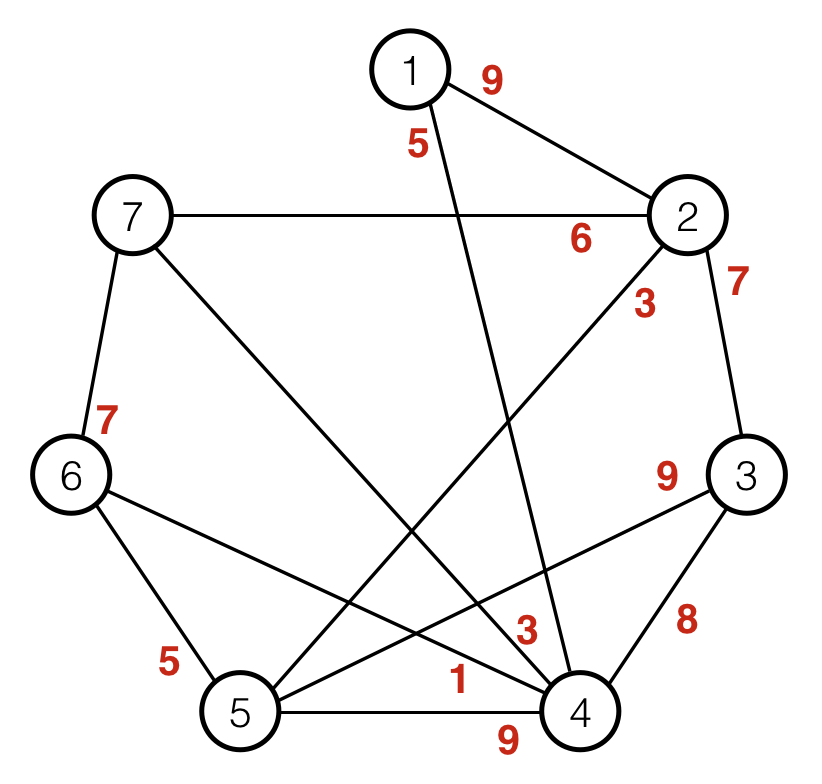
\includegraphics[scale=0.5]{P4.png}
    }
    \end{center}
    Use \textit{Kruskal's Algorithm} to find the maximum-weight spanning tree.

    \paragraph{Initialize}{
        Sort \(\mathit{E}\) by weight from largest to smallest. 
        \[\mathit{E} = \big{\{} (1,2), (3,5), (4,5), (3,4), (2,3), (6,7), (2,7), (1,4), (5,6), (2,5), (4,7), (4,6)\big{\}}\]
        Set \(\mathit{T}=\emptyset\)

        \begin{enumerate}{
            \item \(\mathit{T} \cup \{ (1,2) \} \), cycle free, \(\mathit{T} = \mathit{T} \cup \{ (1,2) \} \)
            \item \(\mathit{T} \cup \{ (3,5) \} \), cycle free, \(\mathit{T} = \mathit{T} \cup \{ (3,5) \} \)
            \item \(\mathit{T} \cup \{ (4,5) \} \), cycle free, \(\mathit{T} = \mathit{T} \cup \{ (4,5) \} \)
            \item \(\mathit{T} \cup \{ (3,4) \} \), cycle!
            \item \(\mathit{T} \cup \{ (2,3) \} \), cycle free, \(\mathit{T} = \mathit{T} \cup \{ (2,3) \} \)
            \item \(\mathit{T} \cup \{ (6,7) \} \), cycle free, \(\mathit{T} = \mathit{T} \cup \{ (6,7) \} \)
            \item \(\mathit{T} \cup \{ (2,7) \} \), cycle free, \(\mathit{T} = \mathit{T} \cup \{ (2,7) \} \)
            \item \(\mathit{T} \cup \{ (1,4) \} \), cycle! No alone vertex, means rest edges make cycle, algorithm end.
        }
        \end{enumerate}
        So that the \(\mathit{T} = \{ (1,2), (3,5), (4,5), (2,3), (6,7), (2,7)\} \)

        The weight of the maximum-weight spanning tree is
        \[\mathit{w}_{1,2}+\mathit{w}_{3,5}+\mathit{w}_{4,5}+\mathit{w}_{2,3}+\mathit{w}_{6,7}+\mathit{w}_{2,7} = 47\]
    }
}

\section*{Question 5}{
    \subsection*{a.}{
        \[\lvert \mathit{B} \rvert = \mathrm{\frac{15 \times 3 + 18 \times 5 + 12 \times 15}{1+2+4} = 45}\]
    }
    \subsection*{b.}{
        The maximum cardinality matching in this graph is 45. \\

        If graph \( \mathit{G} = (\mathit{A} \cup \mathit{B}, \mathit{E})\) has a \textit{Perfect Matching}, which has \(\nu (\mathit{G}) = \lvert \mathit{A} \rvert\), the maximum cardinality matching will be \textit{Perfect Matching}. 

        Now prove that in this case \( \mathit{G} = (\mathit{A} \cup \mathit{B}, \mathit{E})\) has a \textit{Perfect Matching}.

        According to \textit{Theorem 3 (Frobeiniu(1971), Hall(1935))}, only need to prove, 
        \[\lvert \mathit{S} \rvert \leqslant \lvert \mathit{N(S)} \rvert \quad \text{for all} \quad \mathit{S} \subseteq \mathit{A}\]

        Proof by contradiction. If \(\exists \lvert \mathit{S} \rvert > \lvert \mathit{N(S)} \rvert, \mathit{S} \subseteq \mathit{A}\). Suppose that \(\mathrm{k} = \lvert \mathit{S} \rvert, \mathrm{m} = \lvert \mathit{N(S)} \rvert\), i.e. \(\mathrm{k} > \mathrm{m}\). 

        Suppose that \[\mathit{k}_{\mathrm{1}} + \mathit{k}_{\mathrm{2}} + \mathit{k}_{\mathrm{3}} = \mathit{k} > \mathit{m}\]

        in which \(\mathit{k}_{\mathrm{1}}\) refers the number of vertices of degree 3, \(\mathit{k}_{\mathrm{2}}\) refers the number of vertices of degree 5, \(\mathit{k}_{\mathrm{3}}\) refers the number of vertices of degree 15.

        According to the defination of \(\mathit{B}\), we could get \(\mathit{m} \geqslant \mathrm{3}\mathit{k}_{\mathrm{1}}\), \(\mathit{m} \geqslant \mathrm{\frac{5}{2}}\mathit{k}_{\mathrm{2}}\), \(\mathit{m} \geqslant \mathrm{\frac{15}{4}}\mathit{k}_{\mathrm{3}}\), so we have 

        \[\mathit{m} = \mathrm{(\frac{1}{3} + \frac{2}{5} + \frac{4}{15})}\mathit{m} \geqslant \mathit{k}_{\mathrm{1}} + \mathit{k}_{\mathrm{2}} + \mathit{k}_{\mathrm{3}} = \mathit{k} > \mathit{m}\]

        Which makes \(\mathit{m} > \mathit{m}\), \textbf{contradiction}.

        So graph \( \mathit{G} = (\mathit{A} \cup \mathit{B}, \mathit{E})\) has a \textit{Perfect Matching}, and \(\nu (\mathit{G}) = \lvert \mathit{A} \rvert\).
    }
}

\section*{Question 6}{

}

\section*{Question 7}{

}

\section*{Question 8}{

}

\section*{Question 9}{

}

\section*{Question 10}{
    \[\mathcal{B}+\mathcal{F}\]
}



\end{document}
